\chapter*{Introduction}

Façonnée par des millions d'années d'évolution, la nature présente une incroyable diversité de systèmes qui s'adaptent à leur environnement par l'échange, le stockage et le traitement d'information.
Considérée comme un système computationnel, la nature présente ainsi des capacités de calcul extrêmement performantes et efficaces. La conception de systèmes de calculs bio-inspirés part de ce constat de performance et cherche à implémenter certains mécanismes observés dans la nature.
La bio-inspiration a fait ses preuves en intelligence artificielle, robotique ou optimisation. De nombreux algorithmes d'optimisation se sont ainsi inspirés des colonies de fourmis, des essaims d'abeilles, des bancs de poissons ou des chauves-souris, tous ces groupes d'animaux présentant des stratégies de communication efficaces pour accomplir une tâche donnée~\parencite{Darwish2018BioinspiredCA}.
De plus, la recherche en biologie ne cesse d'évoluer, amenant avec elle de nouvelles possibilités d'inspiration biologique.

Le cerveau, vu comme un système computationnel, est un des systèmes les plus complexes que nous connaissons.
Aussi l'inspiration biologique occupe une place de premier rang dans la recherche en intelligence artificielle. Les premiers modèles d'apprentissage s'appuyaient par exemple sur des modèles mathématiques simplifiés de neurones biologiques, tels que \cite{McCulloch1990ALC} et ont conduit à la conception du perceptron, à l'origine des réseaux actuels de \emph{Deep Learning}. Les réseaux convolutifs (CNN) \parencite{LeCun1998ConvolutionalNF}, qui ont révolutionné l'apprentissage d'images, se placent également dans une inspiration biologique, s'inspirant de la décomposition du champ visuel et de la hiérarchie de traitement de l'information visuelle observée dans le cerveau.

De nombreux travaux en neurosciences, dont~\cite{binzegger05, Meunier2009HierarchicalMI,sporns_structure_2013,betzel_multi-scale_2017} proposent que le cortex n'est pas hiérarchique, mais une architecture composée de modules auto-organisés.
Ces modules échangent en continu des informations sensorielles collectées par l'organisme. Ces échanges sont réalisés de façon interne, liant des informations sensorielles et des informations de plus haut niveau provenant de différentes parties du cortex et à différentes échelles spatiotemporelles. 
Enfin, bien qu'une hiérarchie de traitement de l'information apparaisse entre certains modules, de nombreux circuits de rétroactions semblent présents à différents niveaux de l'architecture.
Cette propriété de modularité se retrouve dans de nombreux systèmes biologiques \parencite{clune_evolutionary_2013}. Elle présente des avantages en termes de réutilisation, de robustesse aux fautes, de redondance et de traitement local de l'information. Surtout, cette propriété de modularité est à l'origine des comportements collectifs et des structures dynamiques complexes au sein de ces systèmes~\parencite{flake_computational,Siebert2020RoleOM}.
Dans le cerveau, ces structures dynamiques générées par les interactions entre les neurones semblent être à l'origine de l'apprentissage et la prise de décision. 
Ces comportements fascinants motivent la création de systèmes de calcul modulaires bio-inspirés, dans une recherche de mécanismes de calcul émergents.

Prenons le temps de définir la modularité d'un point de vue computationnel. 
Sa définition varie en effet en fonction des disciplines. D'un point de vue des sciences de l'ingénieur, un système modulaire est un système composé de sous-systèmes, les modules, qui peuvent être ajoutés ou supprimés sans impacter la fonction des autres modules.
Il s'agit d'une approche classique de conception de systèmes en sciences de l'ingénieur~: pour résoudre un problème, on le décompose en sous-problèmes, puis on développe des modules visant à résoudre chacun de ces sous-problèmes.
Dans ce cadre, chaque module a une fonction spécifique et contribue à une tâche globale indépendamment des autres modules.
La définition bio-inspirée de la modularité s'attache en priorité aux interactions entre les modules.
Dans cette approche, les modules des architectures sont en interaction continue dans le temps et présentent des boucles de rétroaction. Les interactions sont gérées de façon locale, sans être supervisées par un processus externe. Grâce aux rétroactions, ces architectures sont des systèmes dynamiques.
Le comportement global du système résulte alors de l'interaction entre les modules et non seulement de la somme des comportements des modules pris individuellement~: il s'agit de systèmes complexes.
Dans cette vision bio-inspirée, la fonction de chaque module n'a de sens que par ses interactions au sein de l'architecture.

La création d'architectures d'apprentissage modulaires, inspirées du cerveau, se retrouve sous le nom d'architectures cognitives~\parencite{Kotseruba201840YO}. Il s'agit de développer des réseaux de neurones autonomes, capables de mémoire et de prise de décision de façon non supervisée, en s'inspirant des capacités du cerveau.
Ces architectures cognitives trouvent leur application en robotique autonome.
L'incorporation de mécanismes d'apprentissage au sein d'agents doit en effet prendre en compte l'aspect temporel et continu du flux de donnée entrant, ce qui appelle à la conception d'architectures d'apprentissage capables de prise de décision autonome.
\cite{brooks_sumsumption_85} a par exemple exploité cette approche modulaire avec l'architecture de \emph{subsumption}. L'auteur propose un système artificiel composé de modules ayant une fonction simple, telle que \og avancer \fg{} ou \og éviter un objet \fg{}. Ces modules sont connectés au sein d'une architecture présentant des rétroactions. Il met en évidence que malgré la simplicité de chacun des modules, le robot est capable d'effectuer des tâches plus complexes, comme explorer son environnement ou suivre une trajectoire tout en évitant les obstacles. Ces tâches de décision émergent de l'interaction des modules simples.
Dans cet exemple, les modules ont une structure préétablie et sont différenciés. Nous pouvons enfin imaginer des architectures dont les modules sont a priori indifférenciés et interchangeables et vont se spécialiser dans l'architecture au cours d'un l'apprentissage. 


Finalement, nous entendons par architecture modulaire d'apprentissage une architecture composée d'une multiplicité de sous-systèmes indifférenciés, interchangeables et évoluant dans le temps.
Ils communiquent entre eux par une interface bien définie et présentent des boucles de rétroaction, leur conférant un aspect dynamique. Cette interaction est traitée localement au sein des modules, sans supervision par un processus extérieur.
Nous pensons que cette approche modulaire de l'apprentissage est propice au développement de nouveaux mécanismes émergeant de l'interaction entre les modules.

Dans cette thèse, nous nous intéressons à un modèle d'apprentissage bio-inspiré existant~: les cartes de Kohonen \parencite{Kohonen1982}. Ces modèles d'apprentissage non-supervisé sont caractérisés par leur capacité à représenter des données de façon ordonnée sur un espace de dimension plus faible (typiquement une ou deux dimensions).
L'algorithme d'apprentissage d'une carte auto-organisatrice suit un principe assez simple. Une carte est composée de vecteurs de l'espace d'entrée (prototypes) positionnés sur une grille de faible dimension.
Ils sont initialement distribués aléatoirement dans l'espace d'entrée. 
L'apprentissage est réalisé en présentant les entrées une à une à la carte, en trouvant leur \emph{Best Matching Unit} qui est le prototype le plus proche de l'entrée, puis en déplaçant ce prototype ainsi que ses voisins dans la grille vers l'entrée courante.
\`A l'issue de ce processus d'apprentissage, la grille munie des prototypes est dépliée sur l'espace d'entrée. N'importe quel vecteur de l'espace d'entrée peut être représenté par une position sur la grille.

La littérature autour des cartes de Kohonen est extrêmement fournie, en témoigne la bibliographie étendue réunissant 7717 travaux entre 1981 et 2005, réunie par \cite{Kaski1998BibliographyOS,oja_bibliography_2002,Honkela2009BIBLIOGRAPHYOS}.
Toutefois, elle s'est principalement attachée à l'amélioration des performances des cartes sur des applications d'apprentissage automatique et de fouille de données, comme de la compression d'image ou du clustering~\parencite{kohonen_essentials_2013}.
Nous pensons que leur inspiration biologique, leurs propriétés d'auto-organisation et de représentation en deux dimensions d'un espace complexe, et la simplicité de leurs règles de mise à jour en font des candidates naturelles pour la création d'une architecture modulaire d'apprentissage.
D'une part les cartes auto-organisatrices peuvent être vues comme un modèle très simplifié d'une aire corticale. Leur assemblage en architecture permettrait de pousser cette inspiration biologique au niveau de la structure du cerveau, dont les aires fonctionnelles semblent présenter des rétroactions à différents niveaux.
D'autre part, elles définissent une représentation en faible dimension de l'espace d'entrée, accessible par les positions dans la carte. D'un point de vue computationnel, cette position se place comme une information peu coûteuse à échanger au sein d'une architecture.

L'idée d'architecture modulaire de cartes auto-organisatrices semble donc découler naturellement du modèle. Cette proposition est d'ailleurs formulée par Kohonen dès 1995~:
\begin{quote}
\og Un objectif à long terme de l'auto-organisation est de créer des systèmes autonomes dont les éléments se contrôlent mutuellement et apprennent les uns des autres. De tels éléments de contrôle peuvent être implémentés par des SOMs spécifiques~; le problème principal est alors l'interface, en particulier la mise à l'échelle automatique des signaux entre les modules et la collecte de signaux pertinents comme interface entre les modules. Nous laisserons cette idée aux recherches futures. \fg{}
(Traduit de \cite{Kohonen1995SelfOrganizingM})
\end{quote}

Depuis, bien que des travaux aient proposé des architectures hiérarchiques de cartes auto-organisatrices, peu ont cherché à les assembler en architectures modulaires non hiérarchiques. 
Les travaux réalisés dans notre équipe de recherche se sont attachés à concevoir un modèle d'architecture modulaire exploitant la position du BMU comme interface entre les cartes~\parencite{baheux_towards_2014}.

Cette thèse poursuit le développement de ce modèle et étudie expérimentalement les comportements qui émergent de l'association des cartes en architecture.
L'architecture que nous proposons rejoint l'idée d'implémenter des mécanismes liés à la cognition, tels que l'apprentissage non-supervisé, la prise de décision autonome, l'apprentissage associatif de données multimodales et le traitement de données temporelles, s'inspirant du traitement multisensoriel du cerveau humain. 
Dans cette thèse, nous explorons en particulier la tâche d'apprentissage associatif de données multimodales.
Il s'agit pour l'architecture d'apprendre des relations existant entre des entrées provenant de différents espaces, en plaçant cet apprentissage de relations à un niveau interne à l'architecture. Le but est d'apprendre à la fois une représentation de chaque espace d'entrée et de leurs relations.

\begin{center}
  $\ast$
\end{center}

Cette thèse présente deux problématiques principales entremêlées~: (i)~développer un modèle d'architecture non hiérarchique de cartes auto-organisatrices exploitant l'aspect spatialement ordonné de ce modèle d'apprentissage, et (ii)~élaborer une méthodologie expérimentale et des outils permettant de mettre en évidence et évaluer l'apprentissage associatif qui émerge d'une telle architecture.

\begin{center}
  $\ast$
\end{center}

Le manuscrit est organisé de la façon suivante.
Le chapitre~\ref{chap:architectures} présente un état de l'art des architectures de cartes auto-organisatrices existant dans la littérature. Ces modèles d'architectures sont issus de plusieurs domaines, de l'apprentissage automatique aux neurosciences computationnelles.
Le chapitre propose une revue des modèles principaux en s'attachant à unifier les notations et leurs désignations afin d'identifier les points communs et différences principales de conception de ces modèles.
Cet état de l'art nous permettra de situer le modèle que nous proposons au regard de la littérature existante.

Nous détaillerons au chapitre~\ref{chap:modele} le modèle d'architecture non hiérarchique de cartes auto-organisatrices que nous développons et étudions dans cette thèse, que nous avons appelé CxSOM, pour \emph{Consensus-driven Multi-SOM}. Il s'inscrit dans la continuité de modèles déjà développés dans notre équipe de recherche.
Nous définissons un modèle de carte qui peut être assemblé à volonté, de façon modulaire, en architecture non hiérarchique. Ce modèle utilise la position du Best Matching Unit d'une carte comme seule interface entre les modules, rendant les activités des cartes interdépendantes. Pour gérer les rétroactions, l'apprentissage s'appuie sur une recherche de consensus entre les cartes pour la recherche d'un BMU.
Le chapitre~\ref{chap:relaxation} est une analyse plus approfondie de la recherche de consensus entre les cartes afin de valider ce mécanisme en tant qu'algorithme de choix de BMU pour l'apprentissage.

La thèse porte sur l'analyse expérimentale des comportements d'apprentissage associatif dans des architectures de deux et trois cartes. Le pari de la construction d'une architecture modulaire est de faire émerger des nouveaux comportements et mécanismes de calcul~; aussi faut-il pouvoir les mettre en évidence. Nos travaux se sont vite confrontés à une difficulté de visualisation d'une telle architecture de cartes. Cette thèse met l'accent sur une méthode d'analyse expérimentale de cette architecture modulaire. Nous en tirerons des comportements élémentaires qui serviront à poser les bases de la construction d'architectures plus complexes.
Nous introduisons au chapitre \ref{chap:repr} cette méthode expérimentale et un cadre de représentation des entrées, et proposons une définition de ce que signifie qu'une architecture de cartes encode les entrées et leurs relations.
Nous présentons ensuite au chapitre \ref{chap:analyse} les comportements élémentaires d'apprentissage associatif observés sur des architectures de deux et trois cartes en une dimension, à partir des représentations que nous avons proposées. Nous présenterons en particulier un comportement de prédiction d'entrée, rendu possible par les rétroactions et la dynamique de recherche du BMU présentes dans notre modèle.
Nous explorons au chapitre~\ref{chap:indicateur} des indicateurs numériques d'évaluation de l'apprentissage associatif par l'architecture de cartes, dans le but d'étendre l'analyse du modèle à des architectures plus grandes, qui seraient difficilement représentables graphiquement.
Le chapitre \ref{chap:analyse2D} étend enfin les mécanismes d'apprentissage que nous avons identifiés à des architectures de cartes en deux dimensions, se plaçant comme une étude préliminaire pour saisir la scalabilité du modèle.
Nous conclurons sur les perspectives de développement du modèle CxSOM que mettent en évidence nos travaux.

    \begin{figure*}[b]
        \vspace{1cm}
        \centering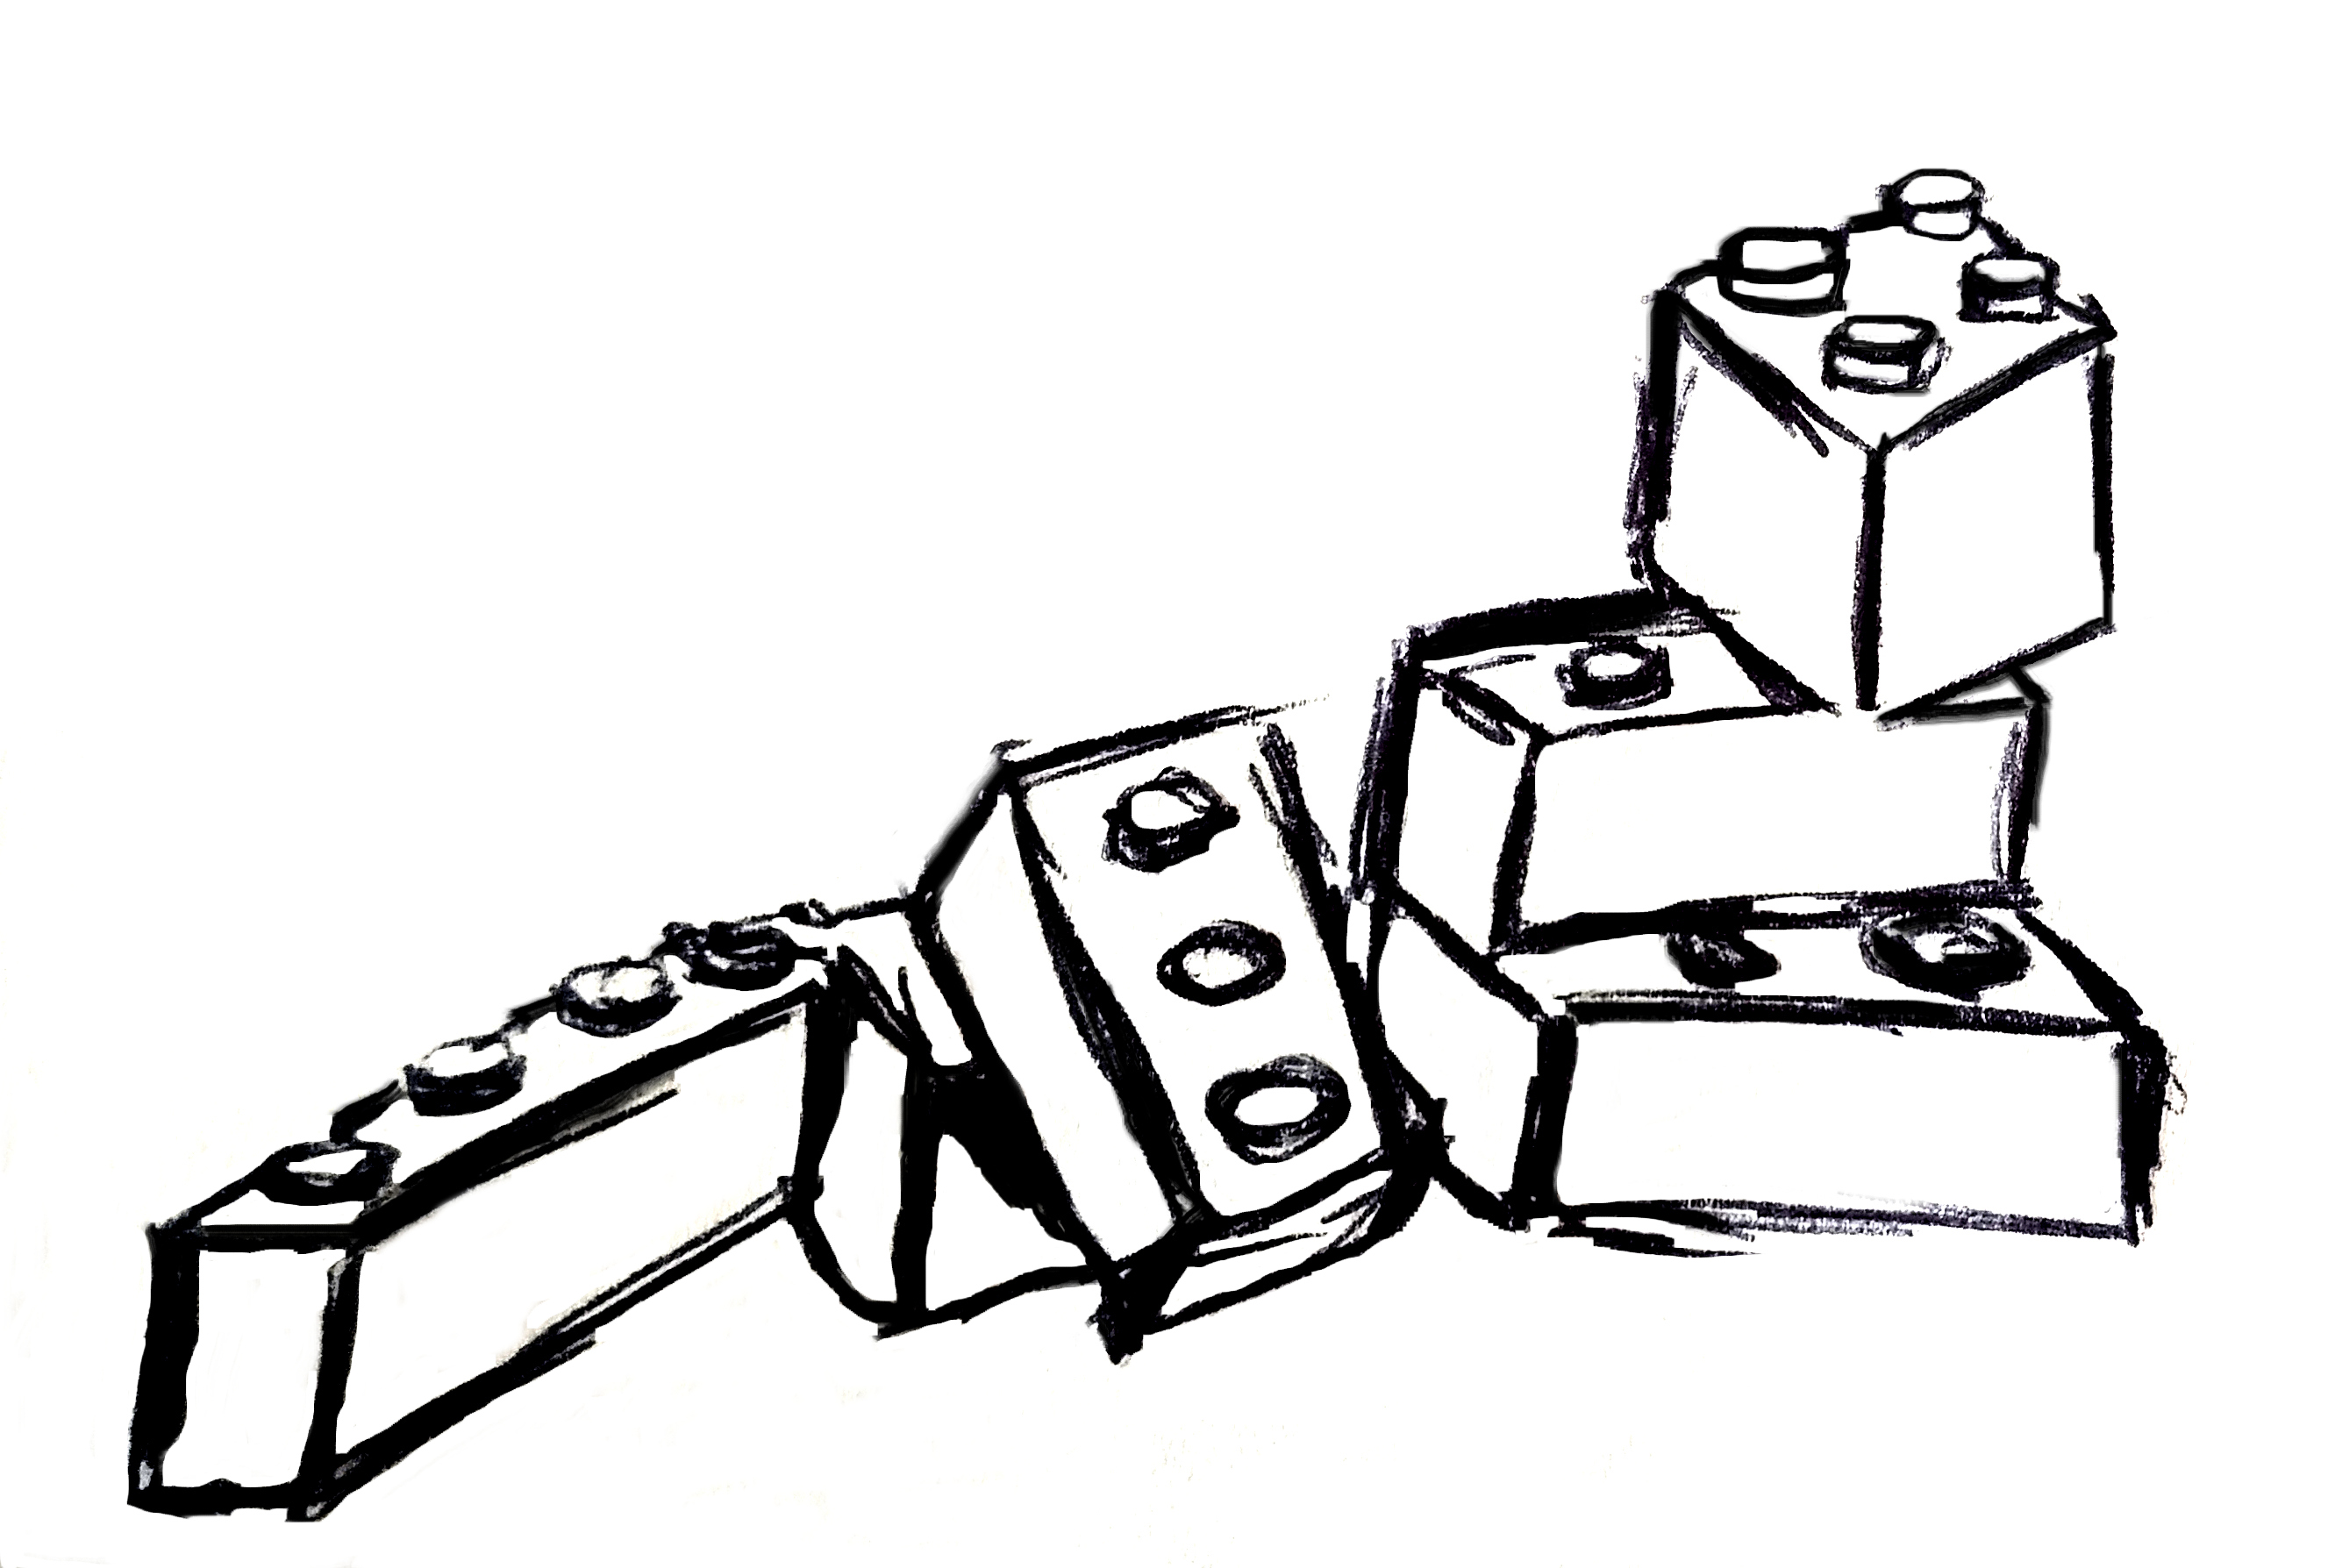
\includegraphics[width=0.3\textwidth]{lego2.jpg}
        \vspace{1cm}
    \end{figure*}

% Idées : plutôt se concentrer sur la SOM en elle-même. Champs d'application, performances, remarquer que les SOM ont des performances pour extraire des représentations, inspi biologique
% Voila ce qui n'a pas été réalisé, et voila ce que je propose : injecter de l'information de position 
% démarche synthétique
% caractériser le comportement émergent des cartes.



% Des systèmes en apparence simples présentent ainsi des capacités d'optimisation de tâches. Le blob est par exemple un être unicellulaire capable de s'étendre sur plusieurs mètres. Uniquement grâce aux communications chimiques opérant au sein de son plasmodium, il est capable de trouver le chemin le plus court dans un labyrinthe entre deux points sur lesquels sont placés de la nourriture \cite{Nakagaki2000IntelligenceMB} ou de retrouver une configuration optimale d'un réseau de transport. Il sont même capables d'apprentissage~: deux entités qui fusionnent se transmettent des connaissances de leur environnement, montrant qu'elles ont chacune emmagasiné, à un point, de l'information sur ce dernier.
% Les colonies de fourmis, quant à elles constituées de milliers, voire de millions d'individus, sont capables de s'auto-organiser pour effectuer des tâches complexes de coopération pour construire leur nid, se défendre face aux prédateurs et trouver leur nourriture via une communication par leurs phéromones, son et toucher.
% Autrement dit, ces systèmes biologiques présentent des capacités de calcul remarquables. 
% Toutes ces stratégies mises en place par des systèmes biologiques ont inspiré de nombreux algorithmes d'optimisation imitant par exemple les colonies de fourmis, les essaims d'abeilles, les groupes de chats, les bancs de poissons ou encore les baleines, tous ces groupes d'animaux présentant des méthodes de communication décentralisées efficaces pour accomplir une tâche donnée~\cite{Darwish2018BioinspiredCA}.




% Les réseaux de neurones impulsionnels (\emph{Spiking Neural Networks}) sont un exemple de modèle d'apprentissage illustrant une complémentarité récente entre l'approche bio-inspirée et l'approche computationnelle.
% Ces réseaux de neurones ont été développés dès les années 1990~\cite{Maass1996NetworksOS} et s'appuient directement sur le modèle biologique du neurone.
% Ils apparaissent dans de nombreux travaux récents comme une méthode montante dans le domaine de l'apprentissage automatique pour la conception de modèles d'apprentissage moins énergivores et distribués, grâce à la conception d'architectures matérielles neuromorphiques telles que LOIHI \footnote{\url{https://www.intel.com/content/www/us/en/research/neuromorphic-computing.html}}. De nombreux travaux cherchent ainsi à adapter des réseaux de neurones classiques de l'état de l'art dans une version impulsionnelle, faisant ainsi passer les SNN de la biologie au calcul~\cite{Schuman2022OpportunitiesFN}.
% De tels modèles apportent de nouveaux paradigmes de calcul pouvant se combiner avec des approches plus appliquées.
% Nous pensons ainsi qu'il est pertinent de continuer à explorer des modèles d'apprentissage automatique inspirés de la biologie.

%Exemples ?
% Le blob est par exemple un être unicellulaire capable de s'étendre sur plusieurs mètres. Uniquement grâce aux communications chimiques opérant au sein de son plasmodium, il est capable de trouver le chemin le plus court dans un labyrinthe entre deux points sur lesquels sont placés de la nourriture \cite{Nakagaki2000IntelligenceMB} ou de retrouver une configuration optimale d'un réseau de transport. Ils sont même capables d'apprentissage~: deux entités qui fusionnent se transmettent des connaissances de leur environnement, montrant qu'elles ont chacune emmagasiné, à un point, de l'information sur ce dernier.
% Les colonies de fourmis, quant à elles constituées de milliers, voire de millions d'individus, sont capables de s'auto-organiser pour effectuer des tâches complexes de coopération pour construire leur nid, se défendre face aux prédateurs et trouver leur nourriture via une communication par leurs phéromones, son et toucher.

%Le perceptron, modèle à l'origine des réseaux de Deep Learning les plus performants à l'heure actuelle, s'inspirait par exemple d'un modèle de neurone biologique très simplifié~\parencite{McCulloch1990ALC}.
% Les réseaux de neurones impulsionnels (\emph{Spiking Neural Networks}) sont un exemple de modèle d'apprentissage illustrant une complémentarité récente entre l'approche bio-inspirée et l'approche computationnelle. Ces réseaux de neurones inspirés du codage temporel des populations de neurones ont été développé dans les années 90~\parencite{Maass1996NetworksOS}. Il apparaissent cependant dans de nombreux travaux récents comme une méthode montante dans le domaine de l'apprentissage automatique pour la conception systèmes d'apprentissage moins énergivores et distribués grâce à la conception de nouvelles architectures matérielles neuromorphiques telles que LOIHI \footnote{\url{https://www.intel.com/content/www/us/en/research/neuromorphic-computing.html}}.
% %\cite{Yamazaki2022SpikingNN}
% L'inspiration biologique apporte ainsi de nouveaux paradigmes de calcul pouvant se combiner avec des approches plus appliquées, et évoluant avec les progrès techniques et matériels de l'informatique.